
\chapter{Dynamical Obstacle Avoidance Framework}
\label{chapter:framework}
Current collaborative robot arms allow more flexible work cells, where they safely collaborate with human operators augmenting productivity in tasks difficult for traditional automation. However,current solutions for safe interaction simply stopping the robot motion  when a collision is detected. This reduces the productivity in an operational setup in which unintended, safe collisions can happen often. Active contact evasion by the robot arm is desirable so that the production process continues despite regular interferences and path obstructions. In the Factory-in-a-day project dynamic collision avoidance technologies have been developed, including a proximity-sensing robot skin, a reactive path-planning solution and a motion control framework based on proximity sensing which is one of the contributions of this  thesis. These technologies have been integrated into a dynamic-obstacle avoidance framework successfully tested in simulation and laboratory set-ups. This chapter presents the obstacle avoidance solution that is currently being implemented with this framework for a collaborative pick and place application prototype. 

Path planning and motion control are usually formalized as separate problems in robotics though both the problems fundamentally solves what a robot should do next. High dimensional configuration spaces, changing environment and uncertainties does not allow to plan real time motion ahead of time requiring a controller to execute the planned trajectory. The fundamental inability to unify both these problems has led to handle the planned trajectory amidst perturbations and unforeseen obstacles using various trajectory execution and deformation mechanisms. Designing an appropriate architecture to handle the information flow between the control and planning components is also not so trivial. The reactive control using proximity sensors developed is purely an application of the state of the art kinematic Hierarchical Quadratic Programming(HQP) solver to combine both path planning and reactive control within the dynamic collision avoidance framework.


\section{Introduction}
A desire for robotic solutions, particularly in the Small and Medium scale Enterprises (SMEs) is becoming increasingly prominent. Automation and robotics promise to deliver reduction on production costs and increase in productivity. However, traditional automation implies an investment prohibitive for SMEs, whose activities mainly involve small batches of production and high variety of products, for example, due to a seasonal nature of their operations. Concretely, tasks such as assembly, machine filling or packaging, can be automated with a robot in the workcell. However economic feasibility requires to reduce the robotization costs. The Factory-in-a-day project \cite{fiad} tries to reduce the robotization cost by reducing the system integration cost and installation time. The key idea is that the robot solution is flexible so that it can be quickly re-installed and configured to another temporary product line. 

To achieve this flexibility and maintain acceptable levels of productivity, in the Factory-in-a-day approach we propose to automate the easy 80\% of the tasks and leave the hard 20\% for human co-workers. Robot manipulators provide power, repeatability and extended work-space while the human operators provide flexibility and problem solving capacity. In addition, fenceless collaborative robots save space and installation cost. However, this approach requires a very high level of safety and agility; the robots should be aware of any obstacle, including dynamic obstacles such as its humans co-workers, and be able to move to avoid contact. Whereas current co-bots guarantee safe contacts, they degrade the performance of the work cell because of stopping the production. This is one of the breakthrough innovations of the Factory-in-a-day project, robot arms that are aware of all (dynamic) obstacles in their environment, and that respond by moving around these obstacles while still continuing their work.

In this chapter,  Section \ref{sec:framework} presents the framework, its individual components and the connection between them.  Section 2 presents the SOA of collision avoidance.





\section{Framework Components}
\label{sec:framework}
Current collaborative robot solutions guarantee safety, but they use
obstacle detection to stop moving. Our dynamic obstacle avoidance
solution is that of using obstacle detection to respond by moving around the
obstacles while continuing to accomplish the desired tasks. Additionally, the integrated dynamic motion planning approach creates motion
plans that fulfil various task specific constraints for typical industrial
applications. For example the work cell 3D model is used to create a consistent
model of the work environment, so that collision free trajectories are flexibly 
generated for different operations. The automatic consideration of these
constraints  drastically simplifies and speeds-up the deployment of the robot.

An artist's illustration of the proposed dynamic obstacle avoidance solution is shown
in Fig. \ref{fig:overview}. The robot motion control component generates
appropriate motion commands for the robot controller to follow the trajectories required for a given task. The proximity-sensing skin that covers the links and joints of the manipulator, produces information regarding potential collisions. This information is used by the robot motion control
module to adapt the robot motions on the fly to fulfil both constraints:
following the current trajectory (with a certain tolerance) and avoid
collisions. If the collision is unavoidable with local deformations of the
current trajectory, the robot motion control module requests a (global) re-planning,
which is performed on the fly by the reactive path-planner. The motion control
then takes the end effector to the final goal pose using the alternative
trajectory. 

\begin{figure}[t]
\centering
\resizebox{0.8\columnwidth}{!}{\includegraphics{doa/images/overview.png}}
\caption[]{An artist's schematization of the FiaD Dynamic obstacle avoidance
concept is illustrated on the left side. On the right, an overview of the main
components of the solution.}
\label{fig:overview}

\end{figure}

\begin{figure}[h]
\centering
\resizebox{0.8\columnwidth}{!}{\includegraphics{doa/images/sensor_unit.pdf}}
\caption[]{Robot skin developed at Institute for Cognitive Systems (ICS), TUM.}
\label{fig:RobotSkin}
\vspace{-10pt}
\end{figure}	

\subsection{Artificial Robot Skin}
The robot skin system is modularized and transduces multi-modal tactile stimuli \cite{MittendorferYC15}. The robot skin consists of hexagonally shaped PCB modules called skin cells (see Fig. \ref{fig:RobotSkin}). A group of directly connected skin cells is termed skin patch. All skin cells are identical and contain the same set of sensors. The sensors sample 9 tactile stimuli of 4 different modalities, namely vibration (3D acceleration sensor), 3 normal forces (capacitive force sensor), 2 temperatures and 1 distance (optical proximity sensor). These sensors are either off-the-shelf standard ICs or in the case of the force sensors a in-house development. A micro-controller in the back of each skin cell collects data from its sensors, filters it and creates and sends data packets, which contain the most recent values of all sensors. All the skin cells are connected to each other via stretchable flex PCBs which allows the skin to cover curved surfaces and increases its robustness. The network of skin cells is a meshed bidirectional communication network which is routed by the micro-controllers of the skin cells. A self-organized algorithm initializes all the skin cells in a skin network and constructs a bidirectional communication path between each skin cell and the network root, the tactile section unit (TSU). The TSU converts skin network packets to standard UDP Ethernet packets and vice versa. This allows for fast low latency connections between robot skin and PC (see Fig. \ref{fig:SkinCellNetworkArchitecture}).
\begin{figure}[t]
\centering
\resizebox{0.8\columnwidth}{!}{\includegraphics{doa/images/SkinCellNetwork.pdf}}\\[-15pt]
\caption[]{The skin cell network architecture and interface to the PC.}
\label{fig:SkinCellNetworkArchitecture}
\vspace{-10pt}
\end{figure}
The robot skin system also supports the auto-calibration of spatial relationships between skin cells of a skin patch covering a 3D 
surface \cite{Mittendorfer-IROS12tendorfer} such that the kinematic chain of every skin cell to the base frame can easily be determined.  

The proximity sensors used in the skin cells are infrared based sensors. The sensor emits infrared light and captures its reflections on obstacles 
in the range from 0 to 15 cm. The strength of the reflections allows the sensor to estimate the distance between the sensor and detected objects.  

\paragraph{Evaluation of Artificial Robot Skin}
\begin{figure}[h]
\centering
\resizebox{1.0\columnwidth}{!}{\includegraphics{doa/images/Demo.pdf}}\\[-10pt]
\caption[]{Robot TOMM. Its arms and grippers are covered with artificial robot skin. the figure depicts the robot in an industrial scenario.}
\label{fig:TommSorting}
\end{figure}

\begin{figure}[h]
\centering
\resizebox{1.0\columnwidth}{!}{\includegraphics{doa/images/TUD_Setup.JPG}}\\[-10pt]
\caption[]{UR5 setup showing Artificial Skin Cells being activated (with red LEDs) by obstacles ($<= 6\,cm$).}
\label{fig:TUDSetup}
\end{figure}

The \textit{Artificial Robot Skin} (ARS) has been successfully deployed on the robot TOMM \cite{Dean-ICRA17} (see Fig. \ref{fig:TommSorting}). The integration of the multi-modal artificial skin signals in the control loop of the arms is demonstrated in \cite{Dean-Humanoids16} where the self-calibrating artificial skin framework is used to control the dynamic behavior of the industrial robot, e.g. producing compliance in a non-compliant robot. The advantage of these compliant behaviors is to generate safer robots, especially for physical Human-Robot Interaction. The fusion of the multi-modal signals of the artificial skin with different sensors (e.g. cameras and joint encoders) in a semantic level is demonstrated in \cite{Ramirez-Amaro-Humanoids16}. These semantic representations are used to extract general task structures which together with the obtained knowledge can improve and accelerate teaching of new tasks \cite{Dynaov-Humanoids16}. Finally, the integration of these technologies has been evaluated in an industrial scenario, where a human can kinesthetically teach the robot TOMM to sort oranges \cite{Dean-IECON16} (see Fig. \ref{fig:TommSorting}).

ARS has also been deployed successfully on another practical setup with a statically mounted Universal Robots UR5 robot (see Fig. \ref{fig:TUDSetup}). In this setup, the ARS is being used to provide proximity information related to obstacles in the immediate surroundings of the robot.


\section{Reactive Controller}
The motion control is achieved using the Stack of Tasks (SoT) controller
framework \cite{Mansard2009} which employs a hierarchical jacobian control strategy eliminating the analytical inverse kinematics computation thus making it a generic controller for all robot platforms. The controller's hierarchical nature allows the robot to handle multiple kinematic tasks simultaneously exploiting the kinematic redundancy of the robot. The controller's real time capability comes from the high computational speed of the state of the art Hierarchical Quadratic Programming (HQP) solver backing it. 


A \emph{task} basically is a control law that achieves a specific objective which can be a free space task or just an inequality constraint that narrows down the workspace of the robot. The task function formalism is very well discussed in \cite{C.Samson1991}. In the context of our work, tasks generally include robot joint posture task, collision avoidance task, joint limits task and so on. The SoT framework handles the task priorities hierarchically in the real time to ensure there are no conflicts among tasks which is used to achieve dynamic obstacle avoidance without compromising on the main goal.

For example, let us consider a pick and place application in a collaborative
environment. The primary goal for this application is to enable a robot to move
to a (set of) desired pick and place locations repetitively. The pick and place
locations can be defined as posture tasks in SoT. However, a higher priority
task considering the collaborative nature of the environment is to avoid
collisions with obstacles that could be humans, for instance. Typically such a
task is modelled as an ``Inequality'' task and an eventual feasible solution (if
one exists) is computed by the solver by exploiting the kinematic redundancy of the robot. In the jargon of motion planning and control, this behavior is similar to a \emph{local planner}.
However, it is likely that a feasible solution is not found due to the solver
converging to a local minima\footnote{This is caused by the use of task
Jacobians. For further details, please see \cite{Mansard2009}.} In such a
scenario, SoT can also be used to leverage the services of a global planner (see
Section \ref{subsec:react_path}) from the current robot state to the goal so
that an entirely new path is obtained which is free from collisions and
consequently allowing all the specified tasks to be achieved in the order of
their priorities. In Section \ref{sec:prelim_results}, we present the
experimental results of using the SoT controller on a practical setup and in
simulation. The SoT controller has also been configured to work with the ROS-control interface. In all these setups, the proximity information from
the artificial robot skin is used as an input to the collision avoidance task. In
the following part, we briefly present the global path planner software framework
that is used when the SoT controller hits a local minima.
\begin{figure}[t]
\centering
\includegraphics[scale=0.47]{doa/images/architecture_reactive_collision_1.pdf}
% \resizebox{2\columnwidth}{!}{\includegraphics{arch_tom_3}}\\
\caption[]{Dynamic collision avoidance software architecture.}
\label{fig:dca}
\end{figure}

\section{Reactive Motion Planning}
\label{subsec:react_path}
\hypersetup{colorlinks, linkcolor=blue}
The reactive path planning software framework is based on the industry grade KineoWorks\texttrademark\footnote{See
\href{http://www.plm.automation.siemens.com/en\_us/products/open/kineo/kineoworks/index.shtml}{Kineoworks}.} path planning library from Siemens in order to provide fast and reliable robot paths. This framework has also been seamlessly integrated into the ROS-ecosystem via a ROS package called \texttt{kws\_ros\_interface} which provides the planner implementations of KineoWorks as shared objects that are readily usable in ROS-based software via the \texttt{kws\_ros\_planner} ROS node.

Robot kinematic models are provided to KineoWorks in the Unified Robot Description Format (URDF) which is a ROS standard. Furthermore, KineoWorks also accepts the standard ROS representation of a \texttt{PointCloud}\footnote{See http://wiki.ros.org/pcl} for creating collision models of dynamic obstacles in the environment. The point clouds are generated in two ways. In one scenario the point clouds are generated by a standard Kinect 3D camera that is observing the immediate environment of the robot. In the other scenario, the point clouds are generated from the proximity data obtained from the Artificial Skin. Finally, the collision detection for dynamic obstacle avoidance is performed using the Kineo\texttrademark Collision Detector (KCD)\footnote{See \href{http://www.plm.automation.siemens.com/en\_us/products/open/kineo/collision-detector/index.shtml}{KCD}.}. KCD performs 3D collision detection and minimal distance analysis between triangular mesh surfaces in assembly environments. KCD has been designed specifically to minimize memory usage and take advantage of parallel processing. The complete software architecture used for the Dynamic Collision Avoidance capability is shown in Fig. \ref{fig:dca}.


\section{Stack of Tasks}
\label{subsec:sot}
'Stack of Tasks' is a hierarchical jacobian-based task controller framework which implements the generalized inverse kinematic formalism by Hanafusa et Al. for local control of redundant systems\cite{hanafusa1981analysis}\cite{Mansard2009ik}. The framework in the earlier stages implemented the Siciliano's extension to handle multiple equality tasks\cite{siciliano1991general}. It has evolved to handle inequality constraints implementing the state of the art solver. The framework provides a structure that orders actives tasks to compute the control law without compromising on the task priority and control continuity. The framework provides a simple scripting interface to interact with controller components during the runtime and has a wrapper to communicate with the ROS world.
\subsection{State of the Art}
Since a 6-axis robot was designed at Stanford allowing a systematic way to design a robot and compute inverse kinematic solution analytically in the seventies, robots have been widely used for a variety of applications from punching cards and palletizing food items to assembly , welding in big automobile manufacturing lines and intelligent stock handling in warehouses \cite{scheinman1969design}. Safety and reliability became a significantly potential area of research since then \cite{dhillon2012robot}. These robots are usually installed in closed chambers, fixed on the ground and absolute care is taken not to make it operational when the door is open or when the co-worker is around the robot’s workspace {safetyreqs}. The safety guidelines are obviously strict as it is crucial to avoid humans in danger. But things are changing quite rapidly and we have an increased focus on human-robot collaboration with enhanced safety in the last decade \cite{Bicchi2008,dhillon2012robot} driven by creative industrial demands and high interest in flexible mobile manipulators. The safety is evaluated based on various factors influencing the human-robot collision impact such as the proximity distance, relative velocity, robot inertia and so on \cite{Kulic2006}. One of the main requirement is the robot’s capability to perceive the environment and react to it.



%    \begin{figure}[thpb]
%       \centering
%       \includegraphics[scale=0.2]{chapters/doa/images/skin.eps}
%       \caption{A mobile manipulator executing a trajectory to reach a pre-grasp pose while the forearm is approached by a person with his hand. A skin sensor mounted on the forearm is used to sense any obstacle in the proximity. }
%       \label{figurelabel}
%    \end{figure}

Collision avoidance is an essential functionality in terms of safety and it is a well researched topic with various approaches  to handle different scenarios. In the earlier times, the approaches model the obstacles as static entities treating them as a planning problem to avoid collisions \cite{van2011reciprocal}. Replanning is performed based on instantaneous observations if the obstacles are dynamic. These planning based approaches limit the low level control to simple operations with controller frequencies  several times smaller than robot-environment iteration time. Constrained based approaches focus on enhancing low level control to perform complex operations by taking sensor data directly to be reactive enough with the environment \cite{khatib1986real}. The Collision avoidance can be modeled as inequality constraints or tasks in an optimization based controller. There are a variety of possible inequalities both in robot and environment in robot application scenarios. Some examples are joint limits, singularity avoidance, and object tracking in visual servoing. Constraint based robot programming were used extensively to resolve these constraints  locally but were specific to robot and the scenario involved.

Morover  redundant systems are popular due to their increased flexibility of arm and a mobile base to handle inequality constraints. The control of redundant robots is not trivial as it is not always easy to compute  analytic inverse kinematic and dynamic solutions. Task function based approach  resolves redundancy to minimize the error in task space \cite{Samson1991}. They are jacobian based techniques inverting the differential mapping that maps the control space and the error space to compute optimal controller outputs. A systematic framework for redundant system control proposed by Siciliano allowed to execute multiple tasks simultaneously with priorities {siciliano1991general}. These framework can only solve equality tasks and various strategies focuses on transforming inequality constraints to equalities\cite{Nelson95strategiesfor,chan1995weighted,mansard2009directional,raunhardt2007progressive}. These strategies are not generic enough and has priority inversion problems making them unreliable for practical use. 

A cascade approach was alternatively used to represent the inequalities and equalities systematically as a hierarchical least square program[Kanoun 2011] but suffered from computational inefficiencies. Hierarchical quadratic program (HQP) solver uses complete orthogonal decomposition (COD) instead of singular value decomposition (SVD) and an improved search algorithm which makes it more efficient than available solvers \cite{escande2014hierarchical}. Though constraint based approaches are quite an efficient way to handle collisions and a flexibile way to model them, the are merely locally optimal controllers and does not provide a systematic way to escape local minima. This necessitates the support of global path planners to find the optimal path for realizing a robot task. Combining global path planning and a reliable reactive control is an essential need for deploying robots from simple to complex scenarios.

 
\subsection{What is a Task?}
A task basically composes a control law with a specific objective which can be such as reaching a desired joint position, avoiding obstacles in the environment, a visual servoing mechanism for grasping or so on. A task is mainly defined by the error between the desired and current feature, the error jacobian and the gain. These defined tasks are pushed into 'Stack of Tasks' which computes the control law for all the task objectives in an iterative manner\cite{mansard2007task}. 

\[\textit{e(t) = x\textsuperscript{*} - x }\]

where \textit{x} refers to the current state of a feature, \textit{x\textsuperscript{*}} refers to the reference feature.

\subsection{Redundancy Formalism}
Siciliano and Slotine proposed a systematic control framework to compute controller outputs for achieving multiple tasks in redundant systems from the redundancy formalism proposed by Hanafusa et al. The idea is, tasks are solved only in the null space of the higher priority tasks to avoid conflicts with them. This means, a task at any level has no effect on the tasks in the higher level as it uses only the left degrees of freedom. 

Let $(e_{1},J_{1})$ be a primary task  which is defined by  
\begin{equation} \label{eq:tf1}
\dot{e} = J\dot{q} 
\end{equation}
 \textit{J} referring to the Jacobian of the error velocity with respect to joint velocity at the current joint state.


\begin{equation} \label{eq:tf3}
\dot{q} = J_{1}^{+}\dot{e}_{1} + Pz
\end{equation}
 Where \textit{P} is the projector on the null space of the the Jacobian J and \textit{ $z$ } is the arbitrary velocity vector which can be used as a parameter to achieve the secondary objectives. 

Let $(e_{1},J_{1})(e_{2},J_{2})...(e_{n},J_{n})$ be tasks in the stack. The redundancy formalism for two tasks can be extended to n tasks such that $e_{i}$ does not conflict with $e_{j}$ such that $j<i$. 


The recursive joint velocity is of the form
\begin{equation} \label{eq:ntasks}
  \dot{q}_{0} = 0\\
\end{equation}
\begin{equation}
  \dot{q}_{i} = \dot{q}_{i-1}+ (J_{i}P^{A}_{i-1})^{+}(\dot{e}_{i} - J_{i}\dot{q}_{i-1}), i= 1..n
\end{equation}



 where $P^{A}_{i-1}$ is the projector onto the null space of the augmented Jacobian $J_i^A = (J_1...J_i)$ and $\widetilde{J}_i = J_iP_{i-1}^A$ is the limited jacobian of the task. The joint velocity achieving all the task objectives is $\dot{q} = \dot{q}_n$. The recursive projector is computed by 
 
 \[P^A_i = P^A_{i-1} - (J_iP_{i-1}^A)^+J^A_{i-1}  \] 
 
 This systematic way of prioritizing tasks allows simultaneous execution of multiple tasks without conflicting each other.
 \subsection{Hierarchical Quadratic Programming}
Mansard et al. proposed an improved QP solver to manage multiple equality and inequality problems in a prioritized hierarchy to handle redundancies[15]. The solver handles equality tasks quite the same like in Siciliano's framework but the solver uses complete orthogonal decomposition(COD) instead of Sing for solving the least squares which is quite faster and efficient. The Hierarchical complete orthogonal decomposition(HCOD), a COD of the jacobian mapping for all the levels is used to compute primal optimum for all the constraints at once making it computationally faster. 

Kanoun et al. and De lasa et. al used a primal active search algorithm which is very expensive due to inefficient optimal active set search involving inappropriate activation and deactivation of constraints at each level along the cascade\cite{de2010feature}\cite{kanoun2011kinematic}. The HQP solver depends on a modified primal active search algorithm to make the optimal active set computation much more efficient. Lexicographic optimization formalism is introduced to maintain the active set at each iteration consistent with prior levels completely eliminating unnecessary constraint deactivations and activations. The solver is ten times faster than the classical solvers and can consider inequalities at any levels of the
hierarchy \cite{escande2014hierarchical}.
\subsection{Proximity Distance Gradient for Collision Avoidance}
The computation of the gradient of the proximity distance between the collision bodies inspired from \cite{lefebvre2005fast} is required to define inequality constraints in Stack of Tasks to avoid self-collision and with external obstacles using a proximity sensor. Let $d$ be the distance between approximated collision bodies $O_1(q)$ and $O_2(q)$. The distance between these bodies and its variation is mapped to joint actuations $q$. The distance gradient can be computed by:
\[ \frac{\partial d}{\partial q} = n_d^{'}(\frac{\partial o_1(q)}{\partial q}- \frac{\partial o_2(q)}{\partial q}) \]

where $n_d^{'}$ is the unit normal distance vector while $o_1(q)$ and $o_2(q)$ are the respective closest points. The gradient of the closest point $p$ of fixed coordinates $(\rho_1(q),\rho_2(q)....\rho_l(q))$ in the local reference frame $(e_1(q),e_2(q)...,e_l(q))$ of a collision object at joint configuration $q$ is

\[\frac{\partial p}{\partial q} =  \sum_{l=1}^{d}\rho_l(q)\frac{\partial e_l(q) }{\partial q}\]

In a 3 dimensional workspace, the expression can be written as 

\[ \frac{\partial p}{\partial q} =  (x y  z)J_\omega + J_\nu \]

where $J_\omega$ is the jacobian of the rotational degrees of freedom $J_\nu$ is the jacobian of the linear degrees of freedom. In case of the external objects, the second part of the equation can be eliminated if the object is static. 

% This work is a direct application of the HQP solver and a first attempt to combine path planning and reactive control in a jacobian based solver framework eliminating a cumbersome architecture handling the information flow between control and planning components. Stack of Tasks, a controller framework that implements the latest HQP solver is used in this work to apply the proposed methodology. The proposed methodology is tested on PR2, a mobile manipulation platform with a skin sensor mounted on the forearm of the robot to demonstrate the collision avoidance while executing a planned trajectory without compromising the final goal of the scenario. 


% The paper is organised as follows. Section \ref{sec:application} describes the solution for dynamic obstacle avoidance and Section \ref{sec:skin} discusses the proximity-sensing robot skin. In Section \ref{sec:sot} the robot motion control architecture to incorporate the collision information as safety
% constraints to dynamically adapt the trajectory is presented. Section \ref{sec:prelim_results}
% presents the preliminary results obtained in two different robot setups. Finally, in Section \ref{sec:conclusions} we present our concluding remarks and a discussion of the current work in progress.
\paragraph{Combining Path Planning and Reactive Motion Control}
The methodology is based on defining the main goal as a workspace constraint and prioritizing between safety tasks and trajectory execution task (in joint space). The figure \ref{gso} gives an intuitive idea about the stack priority order .
   \begin{figure}[thpb]
      \centering
      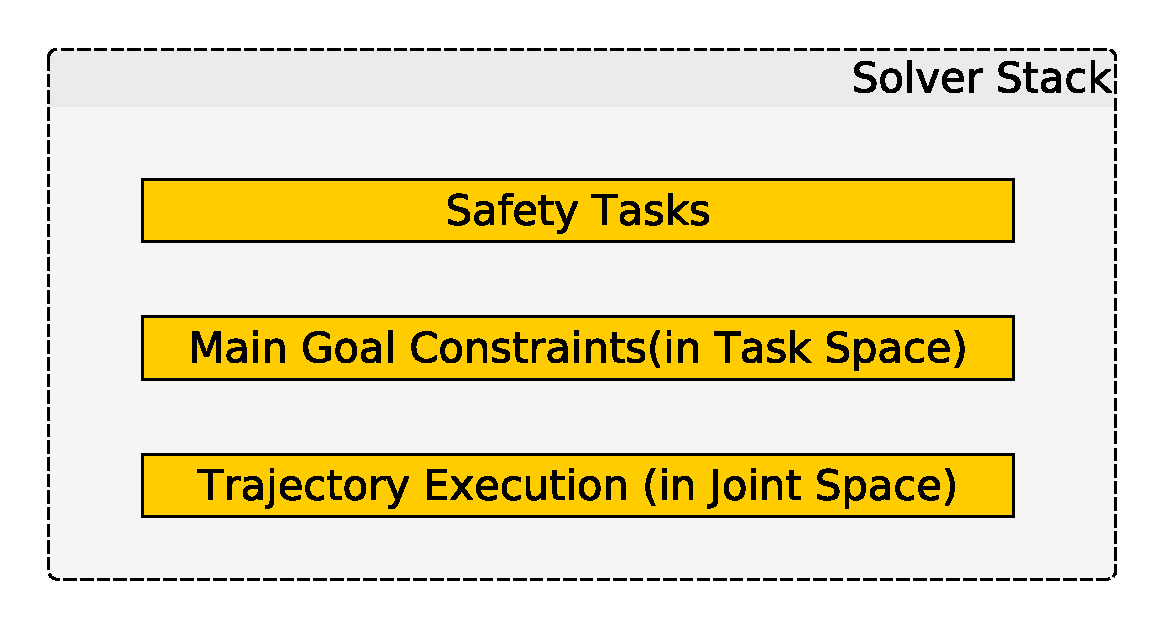
\includegraphics[scale=0.5]{chapters/doa/images/ProposedMethodology.eps}
      \caption{Generic stack order for combining planning and control. }
      \label{gso}
   \end{figure}

Safety tasks are obviously given higher priority in the stack for collision avoidance. Trajectory execution in Joint space occupies the least priority which leaves the controller only the left degrees of freedom from the primary task. If a base trajectory crosses an unforeseen or dynamic obstacle and if the sensors can sense it, the robot basically cannot execute the trajectory until the object is actually moved out of its way. Replanning could be activated if there is no other possibility to reach the joint trajectory goal. Even if there is a possibility to avoid the obstacle and continue executing the  trajectory, it is always not sure that the robot will end up in the desired goal in the task space. The clever trick here is in the way the main goals are defined. The main goal can be moving a base to a particular pose in the world or move the end effector to a grasping pose. Here the important thing is that the goals are something defined in the workspace though a joint trajectory is executed to achieve them. The hierarchical nature of the controller puts this main goal task in high priority and the jacobian core of the solver finds an optimal solution to follow the main goal. The next section illustrates this methodology on a simple scenario to show the potential of this method.


% \section{title}
Current collaborative robot solutions guarantee safety, but they use
obstacle detection to stop moving. Our dynamic obstacle avoidance
solution is that of using obstacle detection to respond by moving around the
obstacles while continuing to accomplish the desired tasks. Additionally, our integrated dynamic motion planning approach creates motion
plans that fulfil various task specific constraints for typical industrial
applications. For example the work cell 3D model is used to create a consistent
model of the work environment, so that collision free trajectories are flexibly 
generated for different operations. The automatic consideration of these
constraints  drastically simplifies and speeds-up the deployment of the robot.

An artist's illustration of our dynamic obstacle avoidance solution is shown
in Fig. \ref{fig:overview}. The robot motion control component generates
appropriate motion commands for the robot controller to follow the trajectories required for a given task. The proximity-sensing skin that covers the links and joints of the manipulator, produces information regarding potential collisions. This information is used by the robot motion control
module to adapt the robot motions on the fly to fulfil both constraints:
following the current trajectory (with a certain tolerance) and avoid
collisions. If the collision is unavoidable with local deformations of the
current trajectory, the robot motion control module requests a (global) re-planning,
which is performed on the fly by the reactive path-planner. The motion control
then takes the end effector to the final goal pose using the alternative
trajectory. The main functional modules of the system are discussed in the following
sections of the paper.

\begin{figure}[t]
\centering
\resizebox{0.8\columnwidth}{!}{\includegraphics{chapters/doa/images/overview}}
\caption[]{An artist's schematization of the FiaD Dynamic obstacle avoidance
concept is illustrated on the left side. On the right, an overview of the main
components of the solution.}
\label{fig:overview}

\end{figure}

\begin{figure}[h]
\centering
\resizebox{0.8\columnwidth}{!}{\includegraphics{figures/sensor_unit}}
\caption[]{Robot skin developed at Institute for Cognitive Systems (ICS), TUM.}
\label{fig:RobotSkin}
\vspace{-10pt}
\end{figure}	

Our robot skin system is modularized and transduces multi-modal tactile stimuli \cite{MittendorferYC15}. 
The robot skin consists of hexagonally shaped PCB modules which we call skin cells (see Fig. \ref{fig:RobotSkin}). 
A group of directly connected skin cells is termed skin patch. All skin cells are identical and contain the same set of sensors.
The sensors sample 9 tactile stimuli of 4 different
modalities, namely vibration (3D acceleration sensor), 3 normal forces (capacitive force sensor), 2 temperatures and 1 distance
(optical proximity sensor). These sensors are either off-the-shelf standard ICs or in the case of the force sensors a in-house development.
A microcontroller in the back of each skin cell collects data from its sensors, filters it and creates and sends data packets,
which contain the most recent values of all sensors. All the skin cells are connected to each other via stretchable flex PCBs 
which allows the skin to cover curved surfaces and increases its robustness. The network of skin cells is a meshed bidirectional
communication network which is routed by the microcontrollers of the skin cells. A self-organized algorithm initializes all 
the skin cells in a skin network and constructs a bidirectional communication path between each skin cell and the network root, 
the tactile section unit (TSU). The TSU converts skin network packets to standard UDP Ethernet packets and vice versa.
This allows for fast low latency connections between robot skin and PC (see Fig. \ref{fig:SkinCellNetworkArchitecture}).
\begin{figure}[t]
\centering
\resizebox{0.8\columnwidth}{!}{\includegraphics{figures/SkinCellNetwork}}\\[-15pt]
\caption[]{The skin cell network architecture and interface to the PC.}
\label{fig:SkinCellNetworkArchitecture}
\vspace{-10pt}
\end{figure}

The robot skin system also supports the auto-calibration of spatial relationships between skin cells of a skin patch covering a 3D 
surface \cite{Mittendorfer-IROS12tendorfer} such that the kinematic chain of every skin cell to the base frame can easily be determined.  

The proximity sensors used in the skin cells are infrared based sensors. The sensor emits infrared light and captures its reflections on obstacles 
in the range from 0 to 15 cm. The strength of the reflections allows the sensor to estimate the distance between the sensor and detected objects.   

\section{Combining motion Planning and control}
There are three kind of paradigms that classifies robot's architecture\cite{asada1986robot}. The first one being the deliberative architectures work on Sense-Plan-Act strategy with environment models to represent the world. They are less reliable for reactivity and human safety because an erroneous representation of world could result in an unfortunate situation. Reactive architectures work on Sense-Act strategy which encompasses the constraint based local controllers on which we had a short look. Though they are reliable for safety, they are only locally optimal and it is impossible to operate independently. The final architecture and the one we are interested is the hybrid architecture that can combine the potential advantages of both the components to successfully realize complex scenarios without compromising safety and reliability. 

The straight forward way to combine both of them is to execute a trajectory and use reactive techniques to take care of safety. If the robot hits a local minimum or a kinematic/task singularity, re-planning mode could be activated. These reactive techniques should basically deform a planned trajectory to achieve the desired goal while taking care of the safety simultaneously. The hierarchical jacobian controller in fact does trajectory deformations which is granted for free by the solver\cite{escande2014hierarchical}. The proposed method actually exploits the hierarchical nature of the solver to perform the deformations without sacrificing the main goal. 

\section{Reactive Control Framework}
The motion control is achieved using the Stack of Tasks (SoT) controller
framework \cite{Mansard2009} which employs a hierarchical jacobian control strategy eliminating the analytical inverse kinematics computation thus making it a generic controller for all robot platforms. The controller's hierarchical nature allows the robot to handle multiple kinematic tasks simultaneously exploiting the kinematic redundancy of the robot. The controller's real time capability comes from the high computational speed of the state of the art Hierarchical Quadratic Programming (HQP) solver backing it. 


A \emph{task} basically is a control law that achieves a specific objective which can be a free space task or just an inequality constraint that narrows down the workspace of the robot. The task function formalism is very well discussed in \cite{C.Samson1991}. In the context of our work, tasks generally include robot joint posture task, collision avoidance task, joint limits task and so on. The SoT framework handles the task priorities hierarchically in the real time to ensure there are no conflicts among tasks which is used to achieve dynamic obstacle avoidance without compromising on the main goal.

For example, let us consider a pick and place application in a collaborative
environment. The primary goal for this application is to enable a robot to move
to a (set of) desired pick and place locations repetitively. The pick and place
locations can be defined as posture tasks in SoT. However, a higher priority
task considering the collaborative nature of the environment is to avoid
collisions with obstacles that could be humans, for instance. Typically such a
task is modelled as an ``Inequality'' task and an eventual feasible solution (if
one exists) is computed by the solver by exploiting the kinematic redundancy of the robot. In the jargon of motion planning and control, this behaviour is similar to a \emph{local planner}.
However, it is likely that a feasible solution is not found due to the solver
converging to a local minima\footnote{This is caused by the use of task
Jacobians. For further details, please see \cite{Mansard2009}.} In such a
scenario, SoT can also be used to leverage the services of a global planner (see
Section \ref{subsec:reactive_path}) from the current robot state to the goal so
that an entirely new path is obtained which is free from collisions and
consequently allowing all the specified tasks to be achieved in the order of
their priorities. In Section \ref{sec:prelim_results}, we present the
experimental results of using the SoT controller on a practical setup and in
simulation. The SoT controller has also been configured to work with the ROS-control interface. In all these setups, the proximity information from
the artificial robot skin is used as an input to the collision avoidance task. In
the following part, we briefly present the global path planner software framework
that is used when the SoT controller hits a local minima.



\subsection{Stack of Tasks}
'Stack of Tasks' is a hierarchical jacobian-based task controller framework which implements the generalized inverse kinematic formalism by Hanafusa et Al. for local control of redundant systems\cite{hanafusa1981analysis}\cite{Mansard2009ik}. The framework in the earlier stages implemented the Siciliano's extension to handle multiple equality tasks\cite{siciliano1991general}. It has evolved to handle inequality constraints implementing the state of the art solver. The framework provides a structure that orders actives tasks to compute the control law without compromising on the task priority and control continuity. The framework provides a simple scripting interface to interact with controller components during the runtime and has a wrapper to communicate with the ROS world.


\subsection{What is a Task?}
A task basically composes a control law with a specific objective which can be such as reaching a desired joint position, avoiding obstacles in the environment, a visual servoing mechanism for grasping or so on. A task is mainly defined by the error between the desired and current feature, the error jacobian and the gain. These defined tasks are pushed into 'Stack of Tasks' which computes the control law for all the task objectives in an iterative manner\cite{mansard2007task}. 

\[\textit{e(t) = x\textsuperscript{*} - x }\]

where \textit{x} refers to the current state of a feature, \textit{x\textsuperscript{*}} refers to the reference feature.

\subsection{Redundancy Formalism}
Siciliano and Slotine proposed a systematic control framework to compute controller outputs for achieving multiple tasks in redundant systems from the redundancy formalism proposed by Hanafusa et al. The idea is, tasks are solved only in the null space of the higher priority tasks to avoid conflicts with them. This means, a task at any level has no effect on the tasks in the higher level as it uses only the left degrees of freedom. 

Let $(e_{1},J_{1})$ be a primary task  which is defined by  
\begin{equation} \label{eq:tf1}
\dot{e} = J\dot{q} 
\end{equation}
 \textit{J} referring to the Jacobian of the error velocity with respect to joint velocity at the current joint state.


\begin{equation} \label{eq:tf3}
\dot{q} = J_{1}^{+}\dot{e}_{1} + Pz
\end{equation}
 Where \textit{P} is the projector on the null space of the the Jacobian J and \textit{ $z$ } is the arbitrary velocity vector which can be used as a parameter to achieve the secondary objectives. 

Let $(e_{1},J_{1})(e_{2},J_{2})...(e_{n},J_{n})$ be tasks in the stack. The redundancy formalism for two tasks can be extended to n tasks such that $e_{i}$ does not conflict with $e_{j}$ such that $j<i$. 


The recursive joint velocity is of the form
\begin{equation} \label{eq:ntasks}
  \dot{q}_{0} = 0\\
\end{equation}
\begin{equation}
  \dot{q}_{i} = \dot{q}_{i-1}+ (J_{i}P^{A}_{i-1})^{+}(\dot{e}_{i} - J_{i}\dot{q}_{i-1}), i= 1..n
\end{equation}



 where $P^{A}_{i-1}$ is the projector onto the null space of the augmented Jacobian $J_i^A = (J_1...J_i)$ and $\widetilde{J}_i = J_iP_{i-1}^A$ is the limited jacobian of the task. The joint velocity achieving all the task objectives is $\dot{q} = \dot{q}_n$. The recursive projector is computed by 
 
 \[P^A_i = P^A_{i-1} - (J_iP_{i-1}^A)^+J^A_{i-1}  \] 
 
 This systematic way of prioritizing tasks allows simultaneous execution of multiple tasks without conflicting each other.
 
\subsection{Hierarchical Quadratic Programming}
Mansard et al. proposed an improved QP solver to manage multiple equality and inequality problems in a prioritized hierarchy to handle redundancies[15]. The solver handles equality tasks quite the same like in Siciliano's framework but the solver uses complete orthogonal decomposition(COD) instead of Sing for solving the least squares which is quite faster and efficient. The Hierarchical complete orthogonal decomposition(HCOD), a COD of the jacobian mapping for all the levels is used to compute primal optimum for all the constraints at once making it computationally faster. 

Kanoun et al. and De lasa et. al used a primal active search algorithm which is very expensive due to inefficient optimal active set search involving inappropriate activation and deactivation of constraints at each level along the cascade\cite{de2010feature}\cite{kanoun2011kinematic}. The HQP solver depends on a modified primal active search algorithm to make the optimal active set computation much more efficient. Lexicographic optimization formalism is introduced to maintain the active set at each iteration consistent with prior levels completely eliminating unnecessary constraint deactivations and activations. The solver is ten times faster than the classical solvers and can consider inequalities at any levels of the
hierarchy \cite{escande2014hierarchical}.
\subsection{Proximity Distance Gradient for Collision Avoidance}
The computation of the gradient of the proximity distance between the collision bodies inspired from \cite{escandestrictly} is required to define inequality constraints in Stack of Tasks to avoid self-collision and with external obstacles using a proximity sensor. Let $d$ be the distance between approximated collision bodies $O_1(q)$ and $O_2(q)$. The distance between these bodies and its variation is mapped to joint actuations $q$. The distance gradient can be computed by:
\[ \frac{\partial d}{\partial q} = n_d^{'}(\frac{\partial o_1(q)}{\partial q}- \frac{\partial o_2(q)}{\partial q}) \]

where $n_d^{'}$ is the unit normal distance vector while $o_1(q)$ and $o_2(q)$ are the respective closest points. The gradient of the closest point $p$ of fixed coordinates $(\rho_1(q),\rho_2(q)....\rho_l(q))$ in the local reference frame $(e_1(q),e_2(q)...,e_l(q))$ of a collision object at joint configuration $q$ is

\[\frac{\partial p}{\partial q} =  \sum_{l=1}^{d}\rho_l(q)\frac{\partial e_l(q) }{\partial q}\]

In a 3 dimensional workspace, the expression can be written as 

\[ \frac{\partial p}{\partial q} =  (x y  z)J_\omega + J_\nu \]

where $J_\omega$ is the jacobian of the rotational degrees of freedom $J_\nu$ is the jacobian of the linear degrees of freedom. In case of the external objects, the second part of the equation can be eliminated if the object is static. 

\section{KINEO}
\hypersetup{colorlinks, linkcolor=blue}
The reactive path planning software framework is based on the industry grade KineoWorks\texttrademark\footnote{See
\href{http://www.plm.automation.siemens.com/en\_us/products/open/kineo/kineoworks/index.shtml}{Kineoworks}.} path planning library from Siemens in order to provide fast and reliable robot paths. This framework has also been seamlessly integrated into the ROS-ecosystem via a ROS package called \texttt{kws\_ros\_interface} which provides the planner implementations of KineoWorks as shared objects that are readily usable in ROS-based software via the \texttt{kws\_ros\_planner} ROS node.

Robot kinematic models are provided to KineoWorks in the Unified Robot Description Format (URDF) which is a ROS standard. Furthermore, KineoWorks also accepts the standard ROS representation of a \texttt{PointCloud}\footnote{See http://wiki.ros.org/pcl} for creating collision models of dynamic obstacles in the environment. In our work, point clouds are generated in two ways. In one scenario the point clouds are generated by a standard Kinect 3D camera that is observing the immediate environment of the robot. In the other scenario, the point clouds are generated from the proximity data obtained from the Artificial Skin. Finally, the collision detection for dynamic obstacle avoidance is performed using the Kineo\texttrademark Collision Detector (KCD)\footnote{See \href{http://www.plm.automation.siemens.com/en\_us/products/open/kineo/collision-detector/index.shtml}{KCD}.}. KCD performs 3D collision detection and minimal distance analysis between triangular mesh surfaces in assembly environments. KCD has been designed specifically to minimize memory usage and take advantage of parallel processing. The complete software architecture used in our paper for the Dynamic Collision Avoidance functionality is shown in Fig. \ref{fig:arch_dca}.
\begin{figure}[t]
\centering
\includegraphics[scale=0.47]{architecture_reactive_collision_1}
% \resizebox{2\columnwidth}{!}{\includegraphics{arch_tom_3}}\\
\caption[]{Dynamic collision avoidance software architecture.}
\label{fig:dca}
\end{figure}

In the following sections we present the current results we have of using the different functionalities described.




\section{Method to combine Path Planning and Reactive Motion Control}
The methodology is based on defining the main goal as a workspace constraint and prioritizing between safety tasks and trajectory execution task (in joint space). The figure \ref{gso} gives an intuitive idea about the stack priority order .
   \begin{figure}[thpb]
      \centering
      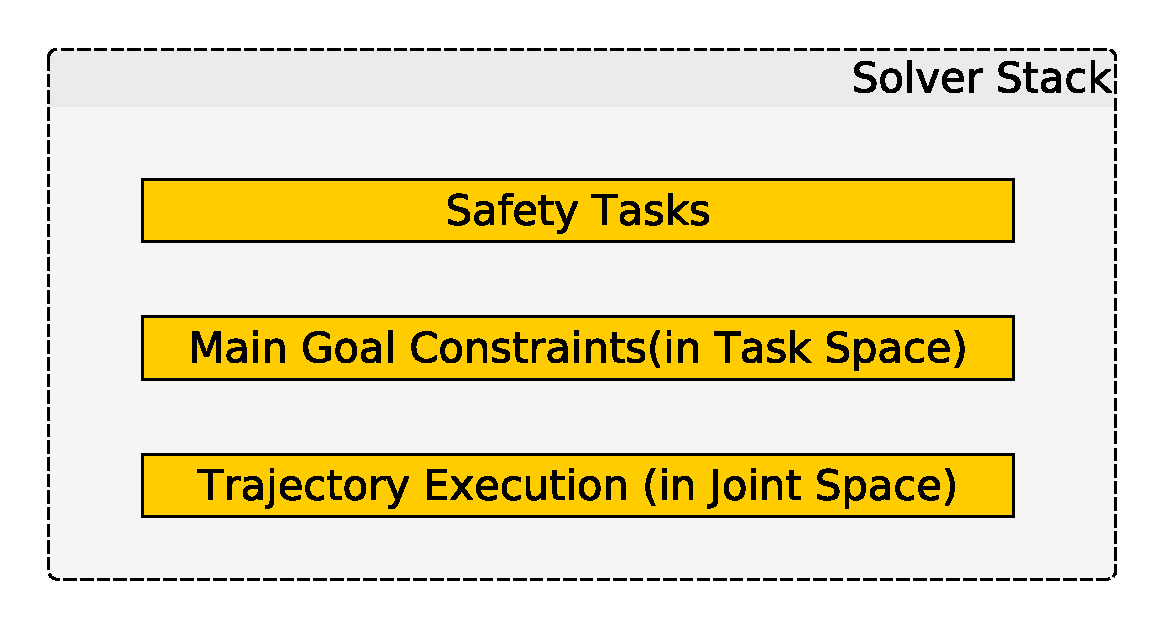
\includegraphics[scale=0.5]{chapters/doa/images/ProposedMethodology.eps}
      \caption{Generic stack order for combining planning and control. The priorities decreases from top to bottom. }
      \label{gso}
   \end{figure}

\begin{itemize}
 \item Safety tasks are obviously given higher priority in the stack for collision avoidance.
 \item Trajectory execution in Joint space occupies the least priority which leaves the controller only the left degrees of freedom from the primary task. If a base trajectory crosses an unforeseen or dynamic obstacle and if the sensors can sense it, the robot basically cannot execute the trajectory until the object is actually moved out of its way. Replanning could be activated if there is no other possibility to reach the joint trajectory goal. Even if there is a possibility to avoid the obstacle and continue executing the  trajectory, it is always not sure that the robot will end up in the desired goal in the task space. 
 
 \item The clever trick here is in the way the main goals are defined. The main goal can be moving a base to a particular pose in the world or move the end effector to a grasping pose. Here the important thing is that the goals are something defined in the workspace though a joint trajectory is executed to achieve them. The hierarchical nature of the controller puts this main goal task in high priority and the jacobian core of the solver finds an optimal solution to follow the main goal. The next section illustrates this methodology on a simple scenario to show the potential of this method.
\end{itemize}


\section{Results}
The Stack of Tasks (SoT) controller has also been deployed and tested for achieving different postures on the setup in Fig. \ref{fig:TUDSetup}. We are actively working on extending the behavior to path following and eventually integrate in accordance with the reactive collision avoidance architecture shown in Fig. \ref{fig:dca}. 


\subsection{Integrated evaluation}
\hypersetup{colorlinks, linkcolor=blue}
The integration of all the components described earlier has been evaluated on a simulation of the orange sorting setup as shown in Fig. \ref{fig:TOMMSimulation}.

\begin{figure}[h]
\centering
\resizebox{1.0\columnwidth}{!}{\includegraphics{doa/images/tomm_simulation.png}}\\[-10pt]
\caption[]{Orange sorting scenario in simulation.The red point cloud is a simulated obstacle.}
\label{fig:TOMMSimulation}
\end{figure}
The evaluation is done in a ROS based gazebo environment with the skin sensors simulated using the flexible collision library to project the distance between objects to sensor range measurements. 
These measurements are mapped to signals compatible in dynamic graph framework using a bridge component to allow its use in the SoT controller. The collision avoidance component computes the point 
distance and jacobian of each and every skin cell configured  essential to feed as an inequality constraint to the solver which backs the SoT controller. The planning component having the capability 
to plan with point cloud data has a Moveit python interface to query motion plan requests. The response is a set of way points which is then linearly interpolated to instantaneous joint position commands
to a path tracking task in the SoT. The SoT controller also has a python interface which makes it easy to design application scenarios.

The combined use of a reactive motion planner and a hierarchical reactive SoT controller with skin data makes it a good candidate for applying dynamical obstacle avoidance in factory environments.
A video result of the same is available \href{https://youtu.be/uLStjR7mpOI}{here}.

% \section{Experimental Illustration}
% We experimented a scenario to verify reactive trajectory execution to achieve a pre-grasp end effector configuration. The SOT framework is embedded in a ROS based real time controller running on a PR2, a mobile manipulation platform. The mobile base and the arms in this platform makes it apt for our scenarios which validates the practical advantage of the proposed methodology. A skin sensor is mounted on the forearm of the left arm . This scenario focuses on executing a simple trajectory on the left arm from an initial position (in the figure \ref{fig:init}) to reach a pregrasp position(in the figure \ref{fig:traj4}). The desired trajectory doesn't involve any movement in joints other than the left arm but they are not constrained to move as a part of the set-up. This figure \ref{ExperimentA} shows the tasks in the stack with priorities decreasing from top to bottom. 
%  The SOT controller executes a preplanned trajectory which is fed to the joint trajectory execution task in the stack. The respective end-effector pose of the trajectory at each instant is fed to an end effector pose task with a priority higher than the joint trajectory task.
%     \begin{figure}[h]
%       \centering
%       \includegraphics[scale=0.21]{doa/images/expillustration.png}
%       \caption{Robot Architecture of the Illustration Scenario}
%       \label{ExperimentA}
%    \end{figure}
 
% The planned way points are fed to a trajectory
% interpolator component which computes instantaneous joint position control
% signals to execute a joint posture task. The skin sensor component being a
% ROS based node publishes topics which are converted to signals in Dynamic
% Graph to be used by collision avoidance component necessary to compute
% information for feeding an inequality task in the solver stack. This is how
% safety and trajectory tracking are executed simultaneously. The adaptability of the controller without compromising the end goal comes
% from the pose task inserted between these tasks. The trajectory interpolator also sends a forward kinematic signal of the end effector corresponding to the joint trajectory point every instant. This allows the controller to stick with the
% plan as close as possible without violating the safety constraints and
% compromising the end goal of the scenario.



% \begin{figure}[!htb]
% \minipage{0.25\textwidth}
%   \includegraphics[width=\linewidth]{doa/images/traj1.png}
%   \caption{Initial Posture}\label{fig:init}
% \endminipage
% \minipage{0.25\textwidth}
%   \vspace{0.15\textwidth}
%   \includegraphics[width=\linewidth]{doa/images/traj4.png}
%   \caption{The robot while executing the trajectory with an actor's hand in proximity.}\label{fig:traj2}
% \endminipage\hfill
% \minipage{0.25\textwidth}%
%   \vspace{0.2\textwidth}
%   \includegraphics[width=\linewidth]{doa/images/traj8.png}
%   \caption{Base motion to avoid proximity with hand simulated yet the wrist pose is maintained.}\label{fig:traj3}
% \endminipage
% \minipage{0.25\textwidth}%
% \vspace{0.13\textwidth}
%   \includegraphics[width=\linewidth]{doa/images/traj11.png}
%   \caption{Final Posture after the sensor error is within the safe region.}\label{fig:traj4}
% \endminipage
% \end{figure}
   
%     \begin{figure}[!h]
%       \centering
%       \includegraphics[scale=0.35]{doa/images/BasePlot-eps-converted-to-crop.pdf}
%       \caption{Base Motion Trajectory Evolution}
%       \label{figurebase}
%    \end{figure}  
   
%   The experiment is done in simulation and the skin sensor error is varied using a software handle. The pink colored vector on the left forearm seen in the figures \ref{fig:init} -\ref{fig:traj4} correspond to unit normal distance vector determining the direction of the robot motion in the workspace to avoid collision. The figure \ref{figurebase} shows the evolution of the base position when the sensor error oscillates between safe and unsafe regions of proximity with an obstacle. They clearly shows the base motion deviating from the reference trajectory but gets back its desired state when the error is in the safe region. The important thing is the pose of the wrist is unchanged except the yaw ( which was relaxed in the pose task to afford base motion to avoid collision while it maintains the pose)
%    \begin{figure}[!h]
%       \centering
%       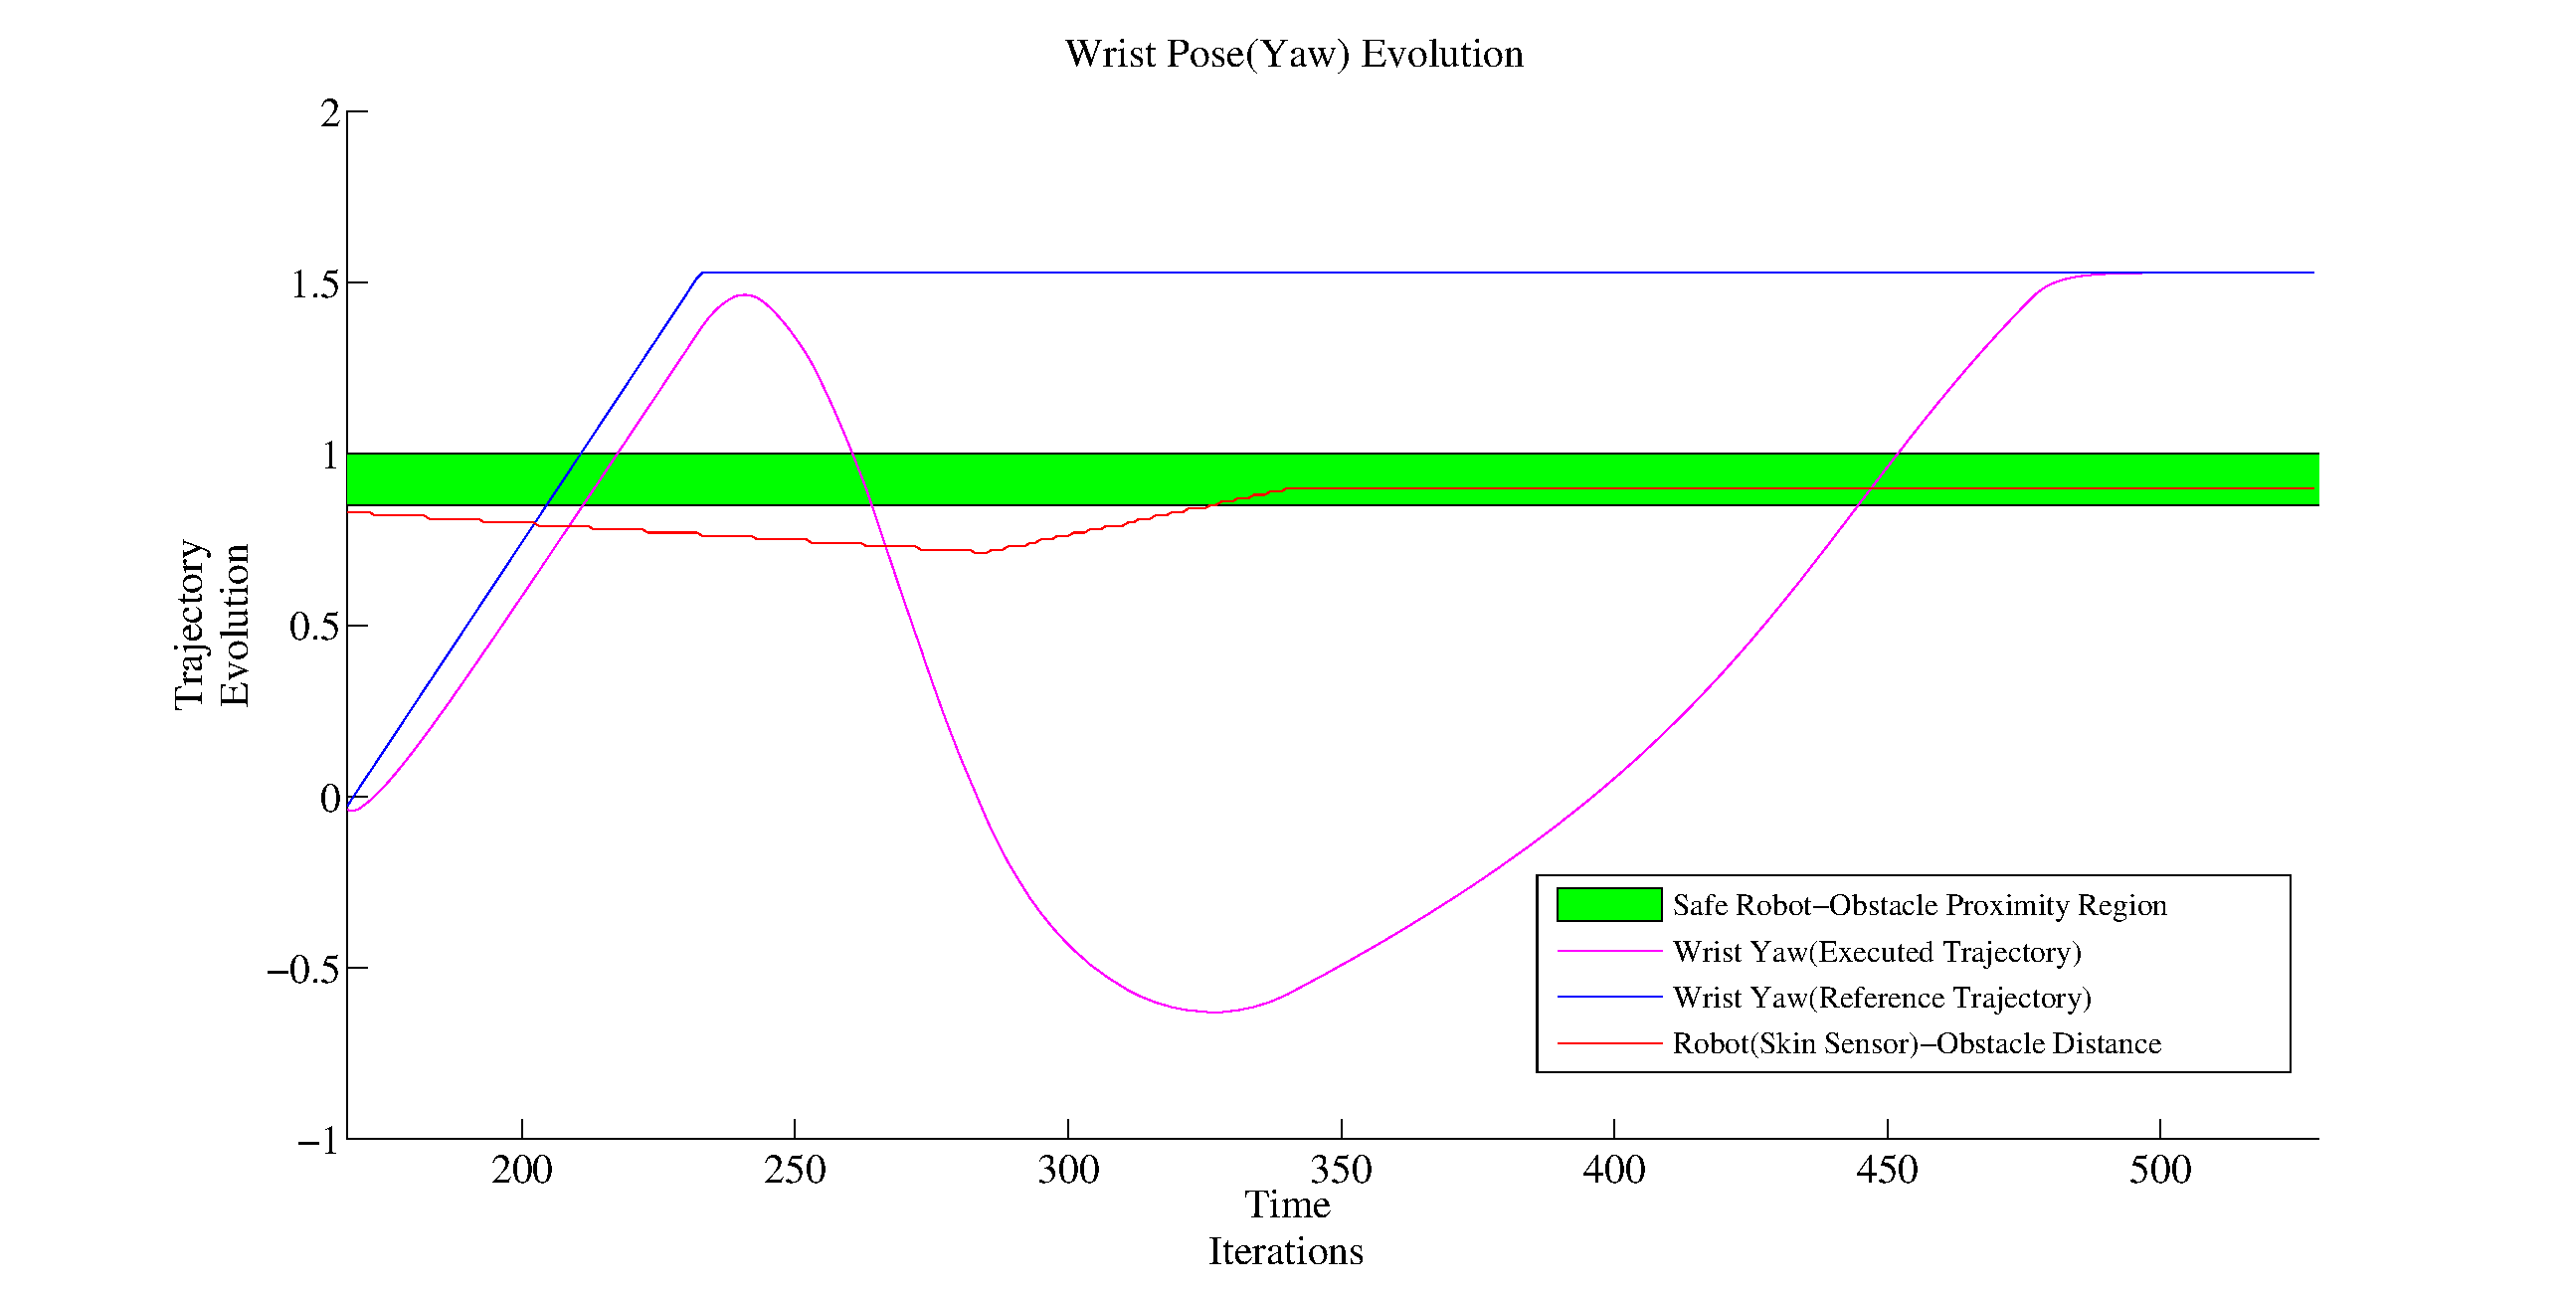
\includegraphics[scale=0.2]{doa/images/WristYawTrajectoryEvolution.eps}
%       \caption{Wrist Pose (Yaw) Evolution}
%       \label{poseYaw}
%    \end{figure}
  
% The figure \ref{poseYaw} shows the evolution of the wrist pose(yaw) of the robot which shows the connection with the base motion to compensate for the collision avoidance but yet the wrist roll and pitch in workspace doesn't change. The simple scenario could be extended to complex scenarios by figuring out the appropriate tasks corresponding to the scenario. The future work will be focused on a generic methodology to generate tasks in the stack just by specifying the scenario and feeding a trajectory.

\section{Conclusion}

This chapter presented the technologies that have been developed in the FiaD
project to augment collaborative robot manipulators with dynamic obstacle
avoidance. All these technologies: a proximity-sensing robot skin, a reactive
path planning solution and a robot motion control strategy, have been validated
in laboratory prototypes. Also, a preliminary prototype of an integrated
solution based on these technologies has been tested in simulation. With the current promising results, we are currently working on a robotic system prototype (based on the setup in Fig. \ref{fig:TUDSetup})

% work in progress%=CITE SUPPORTING EVIDENCE THAT IT WORKS=.
The integration and installation of advanced functionalities such as the dynamic
obstacle avoidance solution presented poses three main challenges from the
software point of view. The first is the integration of different components such as the skin driver, path planner and robot motion control. We address this challenge by adhering to the software development paradigm of the ROS-Industrial initiative. All the components discussed in this paper have been successfully integrated with ROS.

A second challenge is the quality assurance and robustness of the integrated robot software. This is crucial in production environments, and is specially important in collaborative applications, where safety needs to be guaranteed. For this purpose an Automated testing Framework (ATF) has been developed \cite{Weisshardt-2016} as a part of the FiaD prohect, which
allows for the systematic testing of robot software components, which includes unit
 testing, simulation-in-the-loop testing and eventually hardware-in-the-loop testing.
The tests can be automated and integrated in a centralized continuous
integration system. Preliminary test have already been conducted with the
components of the robot software system of this work, and the integrated
prototype applications will be tested with ATF.

Finally, the third challenge is the deployment of the software. One of the main barriers to transfer solutions based on robot frameworks such as ROS to industry, and specially SMEs, is how cumbersome it is
to deploy. As a part of the FiaD project, a Robot deployment toolbox has been developed \cite{Ludtke-2017}, based on ROS, which can also be integrated with ATF.
The deployment tools will also be evaluated on the RBE17 prototype.


% The paper proposed a creative method to execute a trajectory robust to run-time inequality constraints without compromising on the final goal of a scenario. The method uses 'Stack of Tasks', a jacobian control framework employing the state of the art HQP solver for both equality and inequality constraints. The creativity lies on the way the hierarchical nature of the solver and flexible task definition of the framework is exploited to combine an intuitive main goal definition and reactive trajectory execution to realize a scenario successfully robustly. Experiments were done to verify the validity of the method on a PR2 robot with a skin sensor(in simulation) mounted on its forearm. Future work will focus on generalizing the method for various kind of tasks and extending the framework to systematically design tasks to be added in the controller stack specific to possible desired scenarios. The methodology has a significant potential to be used for a robot setup with full body skin sensors.
